%
% 1-fundamtenallemma.tex
%
% (c) 2023 Prof Dr Andreas Müller
%
\section{Das Fundamentallemma für Funktionen mehrere Variablen
\label{buch:felder:section:fundamentallemma}}
\kopfrechts{Das Fundamentallemma}
Der Schlüssel für die Umwandlung eines eindimensionalen Variationsproblems
in eine Differentialgleichung war das Fundamentallemma.

%
% Gebiete
%
\subsection{Gebiete}
Variationsprobleme für Funktionen von nur einer Variablen sind auf 
Funktionen auf einem Intervall beschränkt.
Besteht der Definitionsbereich aus mehreren Intervallen, kann jedes
einzelne Intervall unabhängig von allen anderen betrachtet werden.
Für ein Intervall $[x_0,x_1]$ ist auch das Integral einfach zu definieren,
wie es zur Konstruktion des zu minimierenden Funktionals nötig ist.

Für Funktionen von zwei oder mehr Variablen ist bereits die
Festlegung des Definitionsgebietes viel komplizierter.
Sie muss so erfolgen, dass auch die partielle Integration eines
Produktes darauf übertragbar ist.
Diese wurde im eindimensionalen Fall dazu aus dem Integral
über $F\cdot\eta'$ eine Integral über $dF/dx\cdot \eta$ zu
machen, auf welches das Fundamentallemma anwendbar war.

%
% Offene Mengen
%
\subsubsection{Offene Mengen}
Die Ableitung einer Funktion $f$ in einem Punkt $x\in\mathbb{R}$ erfordert,
dass man Funktionswerte in $x$ mit Funktionswerten in Punkten $x+h$
vergleichen kann, wobei $h\in\mathbb{R}^n$ ein beliebiger kleiner Vektor
sein kann.
Die Ableitung einer Funktion ist dann definiert als die lineare
Ersatzfunktion $Df(x)$ mit der Eigenschaft
\[
f(x+h) = f(x) + Df(x)\cdot h + o(h).
\]
Die Ableitung kann also nur dann sinnvoll definiert werden, wenn
Funktion nicht nur im Punkt $x$, sondern auch in einer Umgebung
des Punktes $x$.
Die Ableitung einer Funktion ist daher nur definiert auf einer
offenen Menge im Sinne der folgenden Definition.

\begin{definition}[offene Menge, Gebiet]
Eine Teilmenge $\Omega\subset\mathbb{R}^n$ heisst {\em offen}, wenn es für
\index{offen}%
jeden Punkt $x\in\Omega$ eine $r>0$ gibt derart, dass ein
Ball mit Radius $r$ um den Punkt $x$ ebenfalls in $\Omega$ enthalten
ist:
\[
B_r(x)
=
\{y\in\mathbb{R}^n
\mid
|y-x|<r\}
\subset \Omega.
\]
Eine offene Menge $\Omega\subset\mathbb{R}$ heisst auch ein {\em Gebiet}.
\index{Gebiet}%
\end{definition}

%
% Der Rand eines Gebietes
%
\subsubsection{Der Rand eines Gebiets}
Die partielle Integration einer Funktion einer Variablen liefert
neben dem Integralterm auch einen Term, der nur von den Werten der
Funktionen an den Endpunkten des Intervalls abhängt.
Es ist zu erwarten, dass ein ähnliches Prinzip auch für die
Integration von Funktionen mehrere Variablen gilt.
Dazu ist jedoch nötig zu erklären, wie genau der Rand eines
Gebietes zu finden ist.

Der Rand eines Intervalls ist einfach zu finden.
Ein Endpunkt eines Intervalls hat die Eigenschaft, dass sich
auf der einen Seite des Punktes lauter Werte befinden, die zum
Intervall gehören, während auf der anderen Seite nur Werte liegen,
die nicht zum Intervall gehören.
Diese anschauliche Beschreibung appelliert aber an eine Vorstellung
einer Richtung und ist daher nicht direkt übersetzbar.
Sie lässt sich aber noch etwas vereinfachen: ein Endpunkt eines
Intervalls hat beliebig nahe Werte die zum Intervall gehören, und
solche die nicht mehr dazu gehören.
Dies suggeriert die folgende Definition für den Rand eines Gebietes.

\begin{definition}[Rand]
\label{buch:felder:fundamentallemma:def:rand}
Ein Randpunkt eines Gebietes $\Omega\subset\mathbb{R}^n$ ist ein Punkt
$x\in\mathbb{R}^n$ mit der Eigenschaft, dass in jeder noch so kleinen 
Umgebung von $x$ Punkte von $\Omega$ und von $\mathbb{R}^n\setminus\Omega$
liegen.
Ein Randpunkt ist also ein Punkt $x\in\mathbb{R}^n$ mit
\[
B_r(x)\cap \Omega\ne \emptyset
\qquad\text{und}\qquad
B_r(x)\cap (\mathbb{R}^n\setminus \Omega)
\ne \emptyset
\]
für alle $r>0$.
Der Rand $\partial \Omega$ eines Gebietes $\Omega$ ist die Menge
aller Randpunkte von $\Omega$.
\end{definition}

Man beachte, dass ein Gebiet $\Omega$ keine Randpunkte enthält.
Wäre $x$ ein Randpunkt von $\Omega$, dann gibt es einen Radius $r$
derart, dass $B_r(x)\in\Omega$ ist.
Für diesen Radius folgt
\[
B_r(x)\cap (\mathbb{R}^n\setminus\Omega)
=
\emptyset,
\]
im Widerspruch zu Annahme, dass $x$ ein Randpunkt war.
Der Widerspruch zeigt, dass ein Punkt von $\Omega$ kein Randpunkt
sein kann.

Die rein punktmengentopologische 
%
% mandelbrot.tex
%
% (c) 2024 Prof Dr Andreas Müller
%
\begin{figure}
\centering
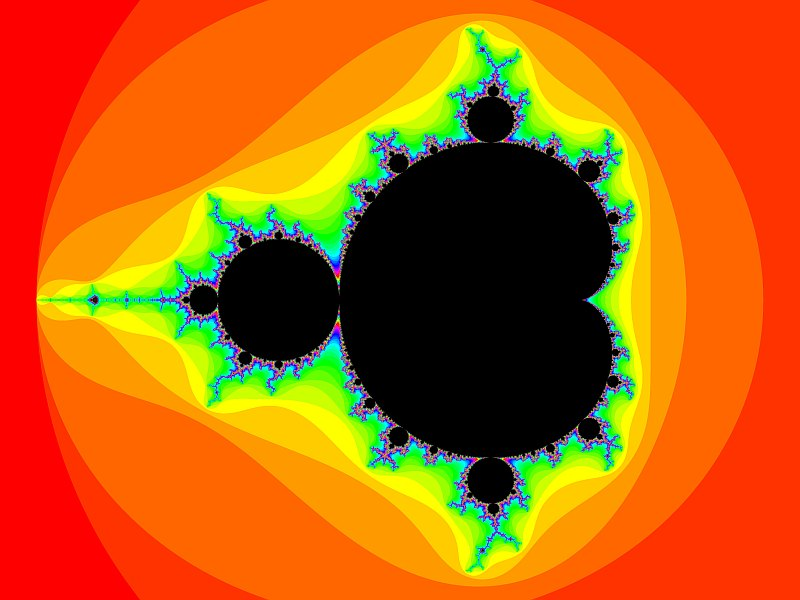
\includegraphics[width=\textwidth]{chapters/040-felder/images/mandelbrot.jpeg}
\caption{Die Mandelbrot-Menge (schwarz) ist berühmt dafür, einen
besonders komplizierten Rand zu haben.
\label{buch:felder:fundamentallemma:fig:mandelbrot}}
\end{figure}
%
Definition~\ref{buch:felder:fundamentallemma:def:rand} des Randes ist
auf Mengen anwendbar, deren Rand sehr kompliziert ist.
Ein Beispiel ist die Mandelbrot-Menge, die in
Abbildung~\ref{buch:felder:fundamentallemma:fig:mandelbrot}
dargestellt ist.
Der schwarze Bereich ist die Mandelbrot-Menge, die farbigen Bereich
liegen ausserhalb der Menge.
Der Rand ist berühmt dafür, dass man beliebig tief hineinzoomen
und immer neue Strukturen entdecken kann.



%
% Integration über ein Gebiet
%
\subsubsection{Integration über ein Gebiet}

%
% Integration über eine Kurve
%
\subsubsection{Integration über eine Kurve}

%
% Integration
%
\subsection{Partielle Integration}
Die partielle Integration für ein Integral einer Variablen
transformiert das Integral
\[
\int_{a}^{b} f(x) g'(x)\,dx
\]
in die Summe
\[
\biggl[ f(x) g(x) \biggr]_a^b
-
\int_a^b f'(x) g(x)\,dx.
\]
Der erste Term hängt nur von Informationen auf dem Rand des 
Definitionsbereichs ab.
Eine Verallgemeinerung dieser Regel muss vor allem auch klären,
wie dieser erste Term aussehen soll.
Er darf nur von den Funktionswerten der Funktionen auf dem Rand
$\partial\Omega$ abhängen.
Die Abhängigkeit muss ausserdem linear sein.
In diesem Abschnitt sollen in einer Folge von Beispielen die
wichtigsten Fälle systematisch entwickelt werden.

%
% Ableitung von Produkten
%
\subsubsection{Ableitung von Produkten}
Die Regel für die partielle Integration von Produkten von Funktionen
einer Variable ist die Integralform der Produktregel
\[
\frac{d}{dx}(f(x)g(x)) = f'(x)g(x) + f(x)g'(x).
\]
Für eine Erweiterung auf ist daher als erstes zu klären, welche Art
von Differentialoperatoren überhaupt in Frage kommen.

Die partielle Ableitung nach einer der Variablen bei Funktionen
$f$ und $g$ von $n$ Variablen erfüllt eine Produktregel:
\[
\frac{\partial}{\partial x_k}
(f(x)g(x))
=
\frac{\partial f}{\partial x_k}(x)\,g(x)
+
f(x)
\,
\frac{\partial g}{\partial x_k}(x)
\]
für jedes $k=1,\dots,n$.
Die partiellen Ableitungen sind aber nur von untergeordnetem Interesse,
da sie für sich allein von der Wahl des Koordinatensystems abhängig 
sind und daher zum Beispiel keine koordinatenunabhängige physikalische
Bedeutung haben können.

Der Gradient wurde aus der Richtungsableitung konstruiert und es wurde
gezeigt, dass 
\[
\operatorname{grad} f(x)
=
\begin{pmatrix}
\frac{\partial f}{\partial x_1}\\
\vdots\\
\frac{\partial f}{\partial x_n}
\end{pmatrix}
\]
eine koordinatenunabhängige Bedeutung als der Vektor hat, in dessen
Richtung die schnellste Zunahme der Funktion $f$ erfolgt.
Und tatsächlich gilt auch für den Gradienten eine Produktformel:
\begin{align*}
\operatorname{grad}(f(x)g(x))
&=
\begin{pmatrix}
\frac{\partial}{\partial x_1}(f(x)g(x))\\
\vdots\\
\frac{\partial}{\partial x_n}(f(x)g(x))
\end{pmatrix}
=
\begin{pmatrix}
\frac{\partial f}{\partial x_1} g(x)
+
f(x) \frac{\partial g}{\partial x_1}\\
\vdots\\
\frac{\partial f}{\partial x_n} g(x)
+
f(x) \frac{\partial g}{\partial x_n}
\end{pmatrix}
\\
&=
(\operatorname{grad}f(x)) g(x)
+
f(x)(\operatorname{grad}g(x))
\end{align*}
Wir haben also den folgenden Satz hergeleitet.

\begin{satz}[Produktformel für Gradient]
Sind $f$ und $g$ Funktionen $\mathbb{R}^n \to\mathbb{R}$, dann gilt
\[
\grad (fg) = (\grad f)g + f\grad g.
\]
\end{satz}

%
% Divergenz
%
\subsubsection{Divergenz}
Der Gradient einer Funktion $f\colon\mathbb{R}^n\to\mathbb{R}$ ist
ein sogenanntes Vektorfeld im Sinne der folgenden Definition.

\begin{definition}[Vektorfeld]
\label{buch:felder:fundamentallemma:def:vektorfeld}
Eine Abbildung $g\colon\mathbb{R}^n\to\mathbb{R}^k$, die jedem Punkt
von $\mathbb{R}^n$ einen $k$-dimensionalen Vektor zuordnet, heisst
ein {\em $k$-dimensionales Vektorfeld}.
\index{Vektorfeld}
\end{definition}

Auch für ein Vektorfeld lassen sich interessante Differentialoperatoren
definieren, deren Bedeutung später klar werden wird.

\begin{definition}[Divergenz]
\label{buch:felder:fundamentallemme:def:divergenz}
Die {\em Divergenz} eines $n$-dimensionalen differenzierbaren
Vektorfeldes $g\colon:\mathbb{R}^n\to\mathbb{R}^n$ ist die Funktion
\[
\operatorname{div} g
\colon
\mathbb{R}^n\to\mathbb{R}
:
x \mapsto
\frac{\partial g_1}{\partial x_1}(x)
+\ldots+
\frac{\partial g_n}{\partial x_n}(x)
=
\sum_{i=1}^n
\frac{\partial g_i}{\partial x_i}(x).
\]
\end{definition}

Auch für die Divergenz gibt es eine Produktformel.
Seien
\[
f\colon\mathbb{R}^3\to\mathbb{R}
\qquad\text{und}\qquad
g\colon\mathbb{R}^3\to\mathbb{R}^3
\]
stetig differenzierbare Funktionen.
Die Komponenten von $g$ schreiben wir $g_i$, $i=1,\dots,n$.

\begin{satz}[Produktformel für Divergenz]
Für 
\[
\operatorname{div}(fg)
=
\grad f \cdot g
+
f\operatorname{div}g.
\]
\end{satz}

\begin{proof}
Wir berechnen die Divergenz von $f\cdot g$:
\begin{align*}
\operatorname{div} fg(x)
&=
\frac{\partial}{\partial x_1}(f(x)g_1(x))
+
\ldots
+
\frac{\partial}{\partial x_n}(f(x)g_n(x))
\\
&=
\frac{\partial f}{\partial x_1}(x)g_1(x)
+f(x)\frac{\partial g_1}{\partial x_1}(x)
+
\ldots
+
\frac{\partial f}{\partial x_n}(x)g_n(x)
+f(x)\frac{\partial g_n}{\partial x_n}(x)
\\
&=
\sum_{i=1}^n \frac{\partial f}{\partial x_i}(x) g_i(x)
+
f(x)
\sum_{i=1}^n \frac{\partial g_i}{\partial x_i}(x)
\\
&=
\grad f(x)\cdot \operatorname{div} g(x)
+
f(x)\operatorname{div}g(x).
\qedhere
\end{align*}
\end{proof}

Die Produktregel sagt also auch hier, dass der Differentialoperator
auf jeden Faktor einzeln angewendet werden kann. 
Je nach Art des Faktors passt aber der Gradient oder die Divergenz.

%
% Laplace-Operator
%
\subsubsection{Laplace-Operator}
Besonderes Interesse an der Divergenz entsteht aus dem Zusammenhang
mit dem Laplace-Operator.

\begin{definition}[Laplace-Operator]
Für eine zweimal stetig differenzierbare Funktion
$f\colon\mathbb{R}^n\to\mathbb{R}$
ist der {\em Laplace-Operator} definiert durch
\[
\Delta f(x)
=
\frac{\partial^2 f}{\partial x_1^2}(x)
+\ldots+
\frac{\partial^2 f}{\partial x_n^2}(x)
=
\sum_{i=1}^n \frac{\partial^2 f}{\partial x_i^2}(x).
\]
\end{definition}

Der Laplace-Operator ist ein Differentialoperator zweiter Ordnung.
Wir berechnen die Zusammensetzung der beiden Differentialoperatorn
erster Ordnung $\operatorname{div}$ und $\grad$
für eine zweimal stetig differenzierbare Funktion
$f\colon\mathbb{R}^n\to\mathbb{R}$ und erhalten
\begin{align*}
\operatorname{div}\grad f(x)
&=
\sum_{i=1}^n
\frac{\partial}{\partial x_i}
\frac{\partial f}{\partial x_i}(x)
=
\frac{\partial^2 f}{\partial x_i^2}(x)
=
\Delta f(x).
\end{align*}
Daraus lässt sich jetzt auch eine Produktformel für den Laplace-Operator
ableiten.
Dazu wenden wir ihn auf das Produkt zweier skalarer Funktionen
$f,g\colon\mathbb{R}^n\to\mathbb{R}$ an:
\begin{align}
\operatorname{div}\grad (fg)(x)
&=
\operatorname{div}\bigl((\grad f(x)) g(x) + f(x)\grad g(x)\bigr)
\intertext{nach der Produktformel für den Gradienten.
Auf die einzelnen Summanden wenden wir jetzt die Produktformel für
die Divergenz an und erhalten}
&=
(\operatorname{div}\grad f(x))g(x) + \grad f(x)\cdot \grad g(x)
\notag
\\
&\qquad\qquad
+
\grad f(x)\cdot\grad g(x) + f(x) \operatorname{div}\grad g(x).
\notag
\intertext{Durch Anwendung der Definition des Laplace-Operators
erhalten wir die gesuchte Produktformel}
\Delta (fg)(x)
&=
(\Delta f(x)) g(x) + 2\grad f(x)\cdot \grad g(x) + f(x)\Delta g(x).
\label{buch:felder:fundamentallemma:eqn:laplaceproduktformel}
\end{align}
Da der Laplace-Operator ein Operator zweiter Ordnung ist, ähnelt 
die rechte Seite von
\eqref{buch:felder:fundamentallemma:eqn:laplaceproduktformel}
der binomischen Formel.

%
% Rotation
%
\subsubsection{Rotation}
In drei Dimensionen gibt es einen weiteren interessanten Differentialoperator,
dessen Konstruktion auf dem Vektorprodukt beruht.

\begin{definition}[Rotation]
Sei $g\colon\mathbb{R}^3\to\mathbb{R}^3$ ein differenzierbares
dreidimensionales Vektorfeld, dann heisst das Vektor
\[
\operatorname{rot}g(x)
=
\begin{pmatrix}
\displaystyle
\frac{\partial g_3}{\partial x_2}
-
\frac{\partial g_2}{\partial x_3}
\\
\displaystyle
\frac{\partial g_1}{\partial x_3}
-
\frac{\partial g_3}{\partial x_1}
\\
\displaystyle
\frac{\partial g_2}{\partial x_1}
-
\frac{\partial g_1}{\partial x_2}
\end{pmatrix}
\]
die {\em Rotation} von $g(x)$.
\end{definition}

Die Rotation $\operatorname{rot}g$ wird im englischen Sprachraum manchmal
auch $\operatorname{curl}g$ geschrieben.
Auch für die Rotation gibt es Produktformeln für die Ableitung.

\begin{satz}[Produktformeln für Rotation]
Sei $f\colon\mathbb{R}^3\to\mathbb{R}$ differenzierbar und
$g,h\colon\mathbb{R}^3\to\mathbb{R}^3$ differenzierbare dreidimensionale
Vektorfelder.
Dann gilt
\begin{align*}
\operatorname{rot}(fg)(x)
&=
\\
\operatorname{rot}(g\times h)(x)
&=
\grad f\times g(x) + f(x)\operatorname{rot}(x).
\end{align*}
\end{satz}

\begin{proof}
Der Beweis erfolgt durch Nachrechnen:
\bgroup
\renewcommand{\arraystretch}{1.9}
\begin{align*}
\operatorname{rot}(fg)(x)
&=
\begin{pmatrix}
\displaystyle
\frac{\partial}{\partial x_2}(fg_3)(x)-\frac{\partial}{\partial x_3}(fg_2)(x)
\\
\displaystyle
\frac{\partial}{\partial x_3}(fg_1)(x)-\frac{\partial}{\partial x_1}(fg_3)(x)
\\
\displaystyle
\frac{\partial}{\partial x_1}(fg_2)(x)-\frac{\partial}{\partial x_2}(fg_1)(x)
\end{pmatrix}
\\
&=
\begin{pmatrix}
\displaystyle
\frac{\partial f}{\partial x_2}(x)g_3(x)
-\frac{\partial f}{\partial x_3}(x)g_2(x)
+
f(x)\biggl(\frac{\partial g_3}{\partial x_2}(x)
-\frac{\partial g_2}{\partial x_3}(x)\biggr)
\\
\displaystyle
\frac{\partial f}{\partial x_3}(x)g_1(x)
-\frac{\partial f}{\partial x_1}(x)g_3(x)
+
f(x)\biggl(\frac{\partial g_1}{\partial x_3}(x)
-\frac{\partial g_3}{\partial x_1}(x)\biggr)
\\
\displaystyle
\frac{\partial f}{\partial x_1}(x)g_2(x)
-\frac{\partial f}{\partial x_2}(x)g_1(x)
+
f(x)\biggl(\frac{\partial g_2}{\partial x_1}(x)
-\frac{\partial g_1}{\partial x_2}(x)\biggr)
\end{pmatrix}
\\[5pt]
&=
(\grad f(x))\times g(x) + f(x)\operatorname{rot}(x).
\qedhere
\end{align*}
\egroup
\end{proof}

%\begin{satz}[Divergenz eines Vektorproduktes]
%\begin{align*}
%\operatorname{div}(g\times h)(x)
%&=
%\end{align*}
%\end{satz}
%
%\begin{proof}
%Durch Nachrechnen
%\begin{align*}
%\operatorname{div}(g\times h)(x)
%&=
%\frac{\partial}{\partial x_1}\bigl(
%g_2(x)h_3(x)-g_3(x)h_2(x)
%\bigr)
%+
%\frac{\partial}{\partial x_2}\bigl(
%g_3(x)h_1(x)-g_1(x)h_3(x)
%\bigr)
%\\
%&\qquad\qquad
%+
%\frac{\partial}{\partial x_3}\bigl(
%g_1(x)h_2(x)-g_2(x)h_1(x)
%\bigr)
%\\
%&=
%\frac{\partial g_2}{\partial x_1}(x)h_3(x)
%-
%g_2(x) \frac{\partial h_3}{\partial x_1}
%+
%\frac{\partial g_3}{\partial x_2}(x)h_1(x)
%-
%g_3(x) \frac{\partial h_1}{\partial x_2}
%\\
%&\qquad\qquad
%+
%\frac{\partial g_1}{\partial x_3}(x)h_2(x)
%-
%g_1(x) \frac{\partial h_2}{\partial x_3}
%\\
%&=
%\frac{\partial g_3}{\partial x_2}(x)h_1(x)
%+
%\frac{\partial g_1}{\partial x_3}(x)h_2(x)
%+
%\frac{\partial g_2}{\partial x_1}(x)h_3(x)
%\\
%&\qquad\qquad
%-
%g_1(x) \frac{\partial h_2}{\partial x_3}
%-
%g_2(x) \frac{\partial h_3}{\partial x_1}
%-
%g_3(x) \frac{\partial h_1}{\partial x_2}
%\\
%&=
%\end{align*}
%\end{proof}

%
% Schreibweise mit dem Nabla-Operator
%
\subsubsection{Schreibeweise mit dem Nabla-Operator}

%
% Der Satz von Green
%
\subsubsection{Der Satz von Green}

%
% Der Satz von Gauss
%
\subsubsection{Der Satz von Gauss}

%
% Der Satz von Stokes
%
\subsubsection{Der Satz von Stokes}

%
% Glatte Funktionen mit kompaktem Träger
%
\subsection{Glatte Funktionen mit kompaktem Träger}

%
% Das Fundamentallemma für mehrere Variablen
%
\subsection{Das Fundamentallemma für mehrere Variablen}
Das Fundamentallemma war instrumental bei der Herleitung der
Euler-Lagrange-Differentialgleichung.
Es besagt, dass eine stetige Funktion von einer Variablen auf einem Intervall
verschwindet, wenn alle ihre Skalarprodukte mit beliebig of stetig
differenzierbaren Funktionen verschwinden.
Diese Eigenschaft gilt auch für Funktionen mehrerer Variablen und kann
ganz analog bewiesen werden.

\begin{satz}[Fundamentallemma]
Sei $\Omega\subset\mathbb{R}^n$ ein Gebiet und $f\colon \Omega\to\mathbb{F}$
eine stetige Funktion.
Ausserdem gelte für jede glatte Funktion $g\colon\Omega\to\mathbb{R}$ 
\begin{equation}
\int_{\Omega} f(x)g(x)\,dx = 0.
\label{buch:felder:fundamentallemma:eqn:bedfundamentallemma}
\end{equation}
Dann folgt $f(x)=0$.
\end{satz}

\begin{proof}
Wie im eindimensionalen Fall kann der Beweis mit einem Widerspruch
geführt werden.
Sei $(x^*_1,\dots,x^*_n)$ ein Punkt im Inneren des Gebietes $\Omega$,
für den $f(x^*_1,\dots,x^*_n)=a\ne 0$ ist.
Da die Funktion $f$ stetig ist, gibt es ein $\delta>0$ derart,
dass sogar
\[
f(x_1,\dots,x_n) > \frac{a}2
\qquad\text{für alle $x_i$ mit $|x_i-x^*_i|<\delta$.}
\]
Da $(x^*_1,\dots,x^*_n)$ im Inneren des Gebietes liegt, kann 
$\delta$ sogar so klein gewählt werden, dass alle Punkte
$(x_1,\dots,x_n)$ mit $|x^*_i-x_n|<\delta$ immer noch in
$\Omega$ liegen.

Sei $h(\xi)$ eine beliebig oft differenzierbare Funktion einer Variablen,
die nur im Intervall $(-\delta,\delta)$ von $0$ verschieden ist und
deren Integral über das Intervall $(-\delta,\delta)$ den Wert $1$ hat.
Mit der Funktion
\[
g(x_1,\dots,x_n)
=
h(x_1-x^*_1)\cdot\ldots\cdot h(x_n-x^*_n),
\]
deren Träger nach Konstruktion in $\Omega$ enthalten ist, wird jetzt das
Integral
\begin{align*}
\int_{\Omega} f(x)\,g(x)\,dx
&=
\int_{\operatorname{supp} g}
f(x)\,h(x_1-x^*_1)\cdots h(x_n-x^*_n)
\,dx_1,\dots,dx_n
\\
&>
\int_{x^*_1-\delta}^{x^*_1+\delta}
\dots
\int_{x^*_n-\delta}^{x^*_n+\delta}
\frac{a}{2}
h(x_n-x^*_n) \,dx_n
\,\dots
h(x_1-x^*_1) \,dx_1
\\
&=
\frac{a}2
\int_{x^*_1-\delta}^{x^*_1+\delta}
h(x_1-x^*_1) \,dx_1
\cdot
\ldots
\cdot
\int_{x^*_n-\delta}^{x^*_n+\delta}
h(x_n-x^*_n) \,dx_n
=
\frac{a}2>0.
\end{align*}
Mit dem konstruierten $g(x)$ ist also eine Funktion gefunden, die
Bedingung~\eqref{buch:felder:fundamentallemma:eqn:bedfundamentallemma}
des Fundamentallemmas nicht erfüllt.
Dieser Widerspruch zeigt, dass die Annahme, $f$ verschwinde nicht überall,
falsch ist.
Damit folgt, dass $f(x)=0$ ist.
\end{proof}



